\documentclass[assignment = 5]{homework}

\usepackage{caption, subcaption, pdfpages, float}
\usepackage{graphics, wrapfig, pgf, graphicx}
\usepackage{enumitem}
\graphicspath{{../resultados/}}


% pacotes para importar código
\usepackage{caption, booktabs}
\usepackage[section, newfloat]{minted}
\definecolor{sepia}{RGB}{252,246,226}
\setminted{
    bgcolor = sepia,
    style   = pastie,
    frame   = leftline,
    autogobble,
    samepage,
    python3,
    breaklines
}
\setmintedinline{
    bgcolor={}
}

% ambientes de códigos de Python
\newmintedfile[pyinclude]{python3}{}
\newmintinline[pyline]{python3}{}
\newcommand{\pyref}[2]{\href{#1}{\texttt{#2}}}

% \SetupFloatingEnvironment{listing}{name=Código}
% \captionsetup[listing]{position=below,skip=-1pt}

\usepackage{csquotes}
\usepackage[style=verbose-ibid,autocite=footnote,notetype=foot+end,backend=biber]{biblatex}
\addbibresource{referencias.bib}
\usepackage[section]{placeins}

\usepackage[hidelinks]{hyperref}
\usepackage[noabbrev, nameinlink, brazilian]{cleveref}
\hypersetup{
    pdftitle  = {MC920 - Trabalho 5 - 187679},
    pdfauthor = {Tiago de Paula}
}

\newcommand{\textref}[2]{
    \hyperref[#2]{#1 \ref*{#2}}
}

\usepackage{import, multirow}
\usepackage{tikz}
\usetikzlibrary{matrix}
\usetikzlibrary{positioning}

\newenvironment{kmatrix}[1][1.3cm]{
    \begin{tikzpicture}[node distance=0cm]
        \tikzset{square matrix/.style={
                matrix of nodes,
                column sep=-\pgflinewidth, row sep=-\pgflinewidth,
                nodes={draw,
                    minimum height=#1,
                    anchor=center,
                    text width=#1,
                    align=center,
                    inner sep=0pt
                },
            },
            square matrix/.default=#1
        }
}{
    \end{tikzpicture}%
}

\newcommand*{\Scale}[2][4]{\scalebox{#1}{\ensuremath{#2}}}%

\newcommand{\red}[1]{\textcolor{red}{\textbf{#1}}}
\def\qm{?}


\begin{document}

    \pagestyle{main}

    \section{Introdução} \label{sec:introducao}


    \section{O Programa} \label{sec:programa}

% TODO: testar 3.6+

A ferramenta foi desenvolvida e testada para as versões de Python 3.6 ou superior. Também foram utilizados os pacotes OpenCV, para entrada e saída de imagens, Numpy, para operações vetorizadas com a imagem, e Matplotlib, para opções de cores para pixels inexistentes.

\subsection{Código-Fonte}

    Neste trabalho foi elaborada a ferramenta \texttt{trasforma.py} que faz a transformação da imagem e aplicação da interpolação. O código responsável pelas operações podem ser encontrados na pasta \texttt{lib}, como apresentado a seguir.

    \begin{description}

        \item[trasnforma.py] Ferramenta de transformação da imagem.

        \item[lib] Conjunto de arquivos com implementações para cada funcionalidade da ferramenta.

        \begin{description}[leftmargin=0\parindent,labelindent=0\parindent]

            \item[idx.py] Criação, transformação e acesso com as coordenadas de cada pixel da imagem.

            \item[linop.py] Operações lineares puras de escalonamento, rotação e translação.

            \item[opimg.py] Operações lineares mais aplicadas a imagem, sempre ajustando o resultado para a origem e retornando as novas dimensões da imagem.

            \item[interp.py] Recuperação da imagem transformada por interpolação dos pontos.

            \item[args.py] Processamento dos argumentos da linha de comando.

            \item[inout.py] Tratamento de entrada e saída de imagens do programa.

            \item[tipos.py] Tipos para checagem estática.
        \end{description}
    \end{description}

    Todas as imagens base para o processamento discutido ao longo do texto estão presente na pasta \texttt{imagens}. Também existe o \textit{script} \texttt{run.sh} em Bash que refaz todos resultados apresentados neste relatório.

\subsection{Execução} % TODO: separar

    A execução de ambos os programas deverá ser feita através do interpretador de Python 3.6+. Os exemplos de execuções a seguir funcionam apenas em Python 3.7+, devido à ordem com que os argumentos são interpretados. No entanto, o \textit{script} \texttt{run.sh} também funciona na versão 3.6.

    O único argumento obrigatório é o caminho da imagem de entrada, preferencialmente PNG, que deverá ser transformada. A imagem de saída é, por padrão, exibida em uma nova janela gráfica, mas pode ser salva em um arquivo com a opção \mintinline{bash}{--output SAIDA} ou \mintinline{bash}{-o SAIDA}.

    A primeira transformação que pode ser feita na imagem é rotação no plano $XY$ por um ângulo $\alpha$. Isso pode ser realizado com \mintinline{bash}{--angulo ALFA} ou \mintinline{bash}{-a ALFA}. Também pode ser feita uma rotação em torno do eixo $Y$, que é projetada em perspectiva para o plano original da imagem. A \textit{flag} para isso é \mintinline{bash}{--beta BETA} ou \mintinline{bash}{-b BETA}. Ambas opções tratam apenas de ângulos em graus.

    % TODO: math eval

    Também temos as opções de escalonamento da imagem. % TODO

    \begin{minted}{bash}
        $ echo MC920 | python3 codificar.py imagens/baboon.png -o saida.png
    \end{minted}

    % TODO: cor

    Todas as opções anteriores estão explicadas com o texto de ajuda da ferramenta, que pode ser acessado com a \textit{flag} \mintinline{bash}{--help} ou apenas \mintinline{bash}{-h}.


    \section{Implementação} \label{sec:implementacao}


    \section{Resultados} \label{sec:resultados}

\subsection{Rotações}

    \begin{figure}[H]
    \centering\hfill
    \begin{subfigure}{0.4\textwidth}
        \centering
        
\includegraphics[width=0.9\textwidth]{rotacoes/16_alp_viz.png}
        \caption{~\texttt{vizinho}.}
    \end{subfigure}%
    \hfill%
    \begin{subfigure}{0.4\textwidth}
        \centering
        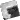
\includegraphics[width=0.9\textwidth]{rotacoes/16_alp_bil.png}
        \caption{~\texttt{bilinear}.}
    \end{subfigure}\hfill
    \\[8pt]\hfill
    \begin{subfigure}{0.4\textwidth}
        \centering
        \includegraphics[width=0.9\textwidth]{rotacoes/16_alp_bic.png}
        \caption{~\texttt{bicubica}.}
    \end{subfigure}%
    \hfill%
    \begin{subfigure}{0.4\textwidth}
        \centering
        \includegraphics[width=0.9\textwidth]{rotacoes/16_alp_lag.png}
        \caption{~\texttt{lagrange}.}
    \end{subfigure}\hfill

    \caption{Rotação de 15\textdegree{} no plano da imagem aplicada em \texttt{house16.png} ($16 \times 16$).}
    \label{fig:house16:alp}
\end{figure}

    \begin{figure}[H]
    \centering
    \begin{subfigure}{0.33\textwidth}
        \centering
        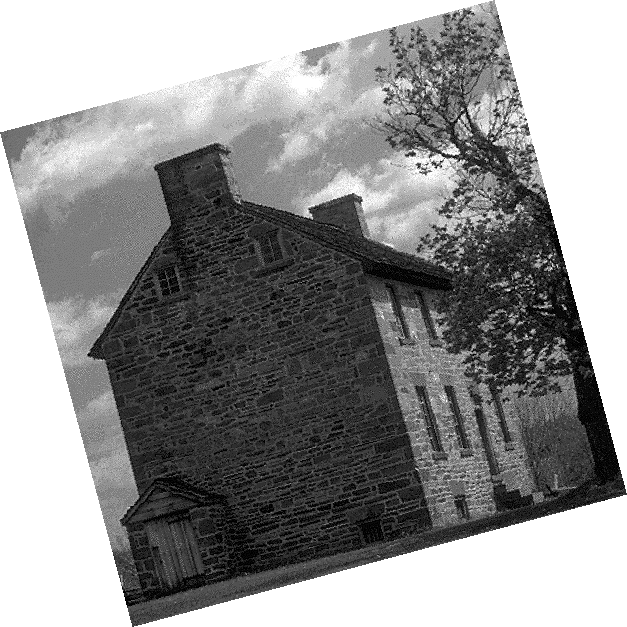
\includegraphics[width=0.9\textwidth]{rotacoes/house_alp_viz.png}
        \caption{~\texttt{vizinho}.}
    \end{subfigure}%
    \hspace{8pt}
    \begin{subfigure}{0.33\textwidth}
        \centering
        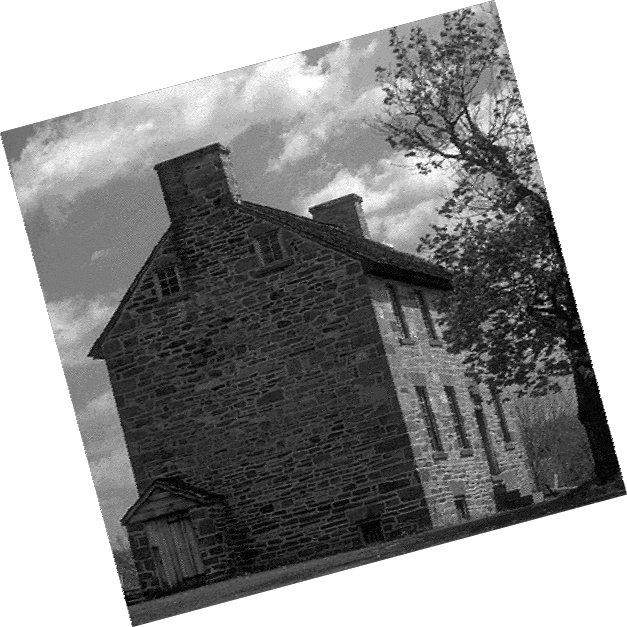
\includegraphics[width=0.9\textwidth]{rotacoes/house_alp_bil.png}
        \caption{~\texttt{bilinear}.}
    \end{subfigure}
    \\[8pt]
    \begin{subfigure}{0.33\textwidth}
        \centering
        \includegraphics[width=0.9\textwidth]{rotacoes/house_alp_bic.png}
        \caption{~\texttt{bicubica}.}
    \end{subfigure}%
    \hspace{8pt}%
    \begin{subfigure}{0.33\textwidth}
        \centering
        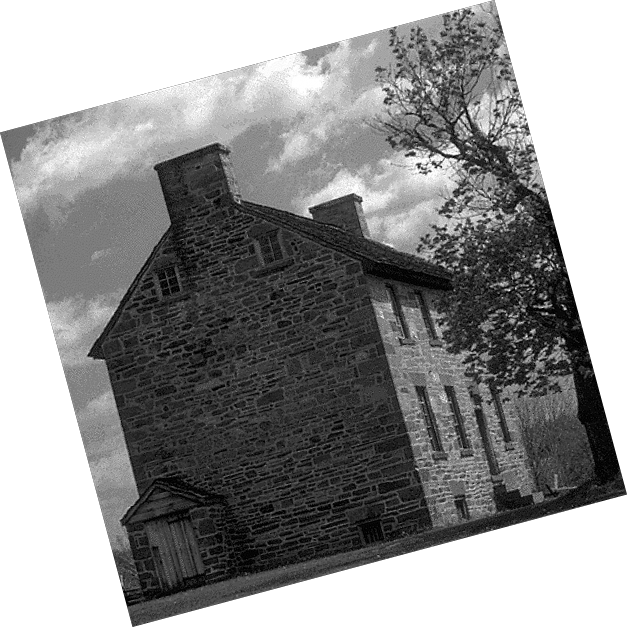
\includegraphics[width=0.9\textwidth]{rotacoes/house_alp_lag.png}
        \caption{~\texttt{lagrange}.}
    \end{subfigure}

    \caption{Rotação de 15\textdegree{} no plano da imagem aplicada em \texttt{house.png} ($512 \times 512$).}
    \label{fig:rot:house}
\end{figure}

    \begin{figure}[H]
    \centering
    \begin{subfigure}{0.3\textwidth}
        \centering
        \includegraphics[width=0.8\textwidth]{rotacoes/64_alp_viz.png}
        \caption{~\texttt{vizinho}.}
    \end{subfigure}%
    \hspace{8pt}%
    \begin{subfigure}{0.3\textwidth}
        \centering
        \includegraphics[width=0.8\textwidth]{rotacoes/64_alp_bil.png}
        \caption{~\texttt{bilinear}.}
    \end{subfigure}
    \\[8pt]
    \begin{subfigure}{0.3\textwidth}
        \centering
        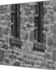
\includegraphics[width=0.8\textwidth]{rotacoes/64_alp_bic.png}
        \caption{~\texttt{bicubica}.}
    \end{subfigure}%
    \hspace{8pt}%
    \begin{subfigure}{0.3\textwidth}
        \centering
        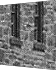
\includegraphics[width=0.8\textwidth]{rotacoes/64_alp_lag.png}
        \caption{~\texttt{lagrange}.}
    \end{subfigure}

    \caption{Rotação de -30\textdegree{} no plano da imagem aplicada em \texttt{house16.png} ($64 \times 64$).}
    \label{fig:rot:house64}
\end{figure}

\subsection{Ampliação}

\subsection{Redução}

\subsection{Reconstrução}

\subsection{Tempo de Execução}


    \section{Conclusão}

Podemos ver que a diferenças dos métodos de interpolação é grande, tanto em relação ao resultado quanto ao tempo necessário para a aplicação. Os métodos mais custosos são os que tem melhores resultados visuais, no caso as interpolações cúbica e por polinômios de Lagrange. No entanto, o método de Lagrange consegue ser melhor em várias situações, por evitar borramento da imagem, mesmo sendo bem mais eficiente.

Em algumas situações, como no caso de \hyperref[sec:escalonamento]{redução das dimensões da imagem}, a interpolação bicúbica pode ser melhor. O método pode ser melhorado ainda mais com algum filtro de frequência, como um de nitidez. Em aplicações como redes neurais, em que \textit{downsampling} é muito importante, esse método pode ser bem útil.

Em outras situações em que \textit{downsampling} também pe necessário, mas não afeta tanto o resultado, a interpolação por vizinho mais próximo pode ser mais interessante. Isso por sua eficiência, capaz de produzir imagens com 20 mega pixels em poucos segundos.


\end{document}
